The dependence of the linearity fit results as a function of  the bunch crossing in the trains is shown in Figures~\ref{fig:fill7358trainresults}.
A systematic drop in the slope is observed as the colliding bunch is farther from the leading bunch.

A check was performed to know if this trend may be caused by the afterglow corrections  as shown in Appendix~\ref{sec:appendix2} where the PCC and HFOC afterglow corrections are removed, however the change in the trend is small.

Comparisons to other luminometers show a similar systematic trend for HFET and BCM1F (Figures~\ref{fig:fill7358trainslope_hfet} and \ref{fig:fill7358trainslope_bcm}).
In the case of PLT (Figure~\ref{fig:fill7358trainslope_plt}) the trend is different and a strong negative slope is obtained for the leading bunch.

The effect was further studied by reprocessing the PCC data while modifying the module veto list to select different parts of the Pixel detector, these results are shown in Figure~\ref{fig:fill7358trainslope_pccparts}.
In these graphs it is observed that BPIX layer 1, FPIX Panel 1 all disks, and FPIX Panel 2 disks 1 show the trend, while the remaining parts are more stable.

\begin{figure}[t]
  \begin{center}
    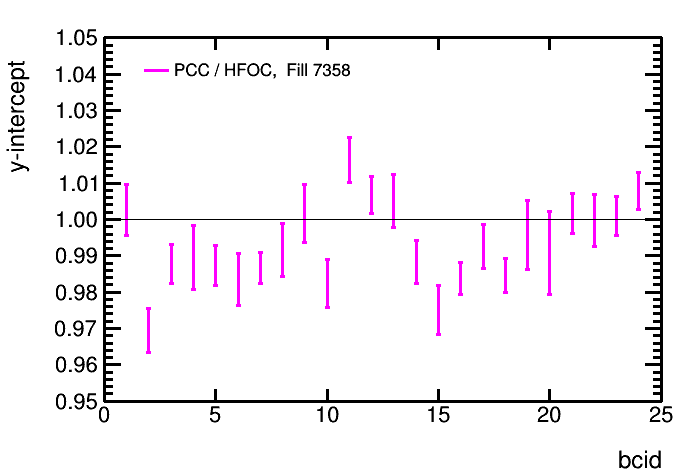
\includegraphics[width=0.47\linewidth]{plots/sbilratios_trains_Fill7358/plot_det_linearity_perbx_y0_7358.png}
    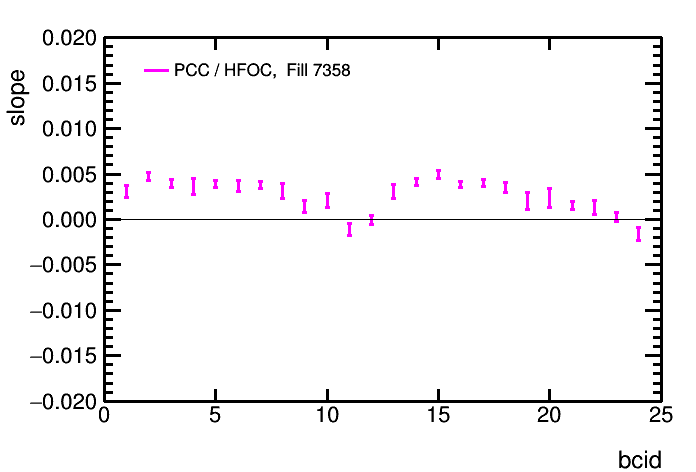
\includegraphics[width=0.47\linewidth]{plots/sbilratios_trains_Fill7358/plot_det_linearity_perbx_slope_7358.png}
    \caption{
      y-intercept and slope values obtained from the linearity fits for the 24 bunches in the two trains of Fill 7358.
      \label{fig:fill7358trainresults}
    }
  \end{center}
\end{figure}



\clearpage
\begin{figure}[t]
  \begin{center}
    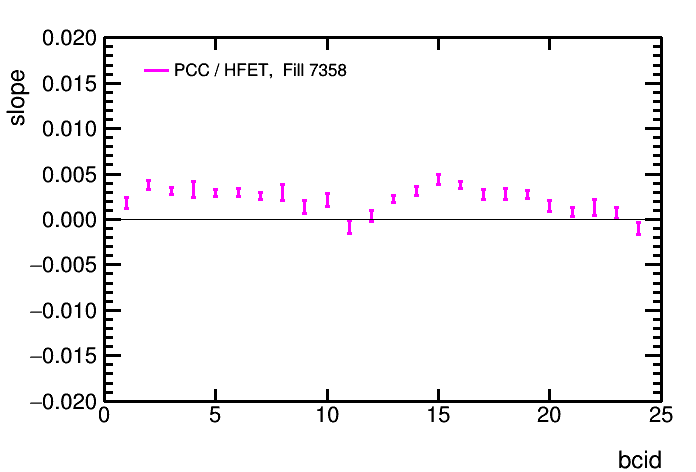
\includegraphics[width=0.47\linewidth]{plots/sbilratios_trains_Fill7358/plot_det_linearity_perbx_slope_7358_hfet.png}
    \caption{
      Slope values obtained from the linearity fits for the 24 bunches in the two trains of Fill 7358, in this plot the PCC is compared to the HFET luminometer.
      \label{fig:fill7358trainslope_hfet}
    }
  \end{center}
\end{figure}

\begin{figure}[t]
  \begin{center}
    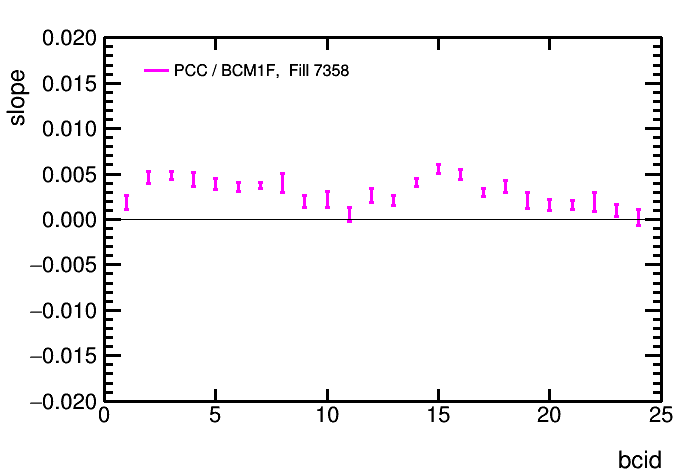
\includegraphics[width=0.47\linewidth]{plots/sbilratios_trains_Fill7358/plot_det_linearity_perbx_slope_7358_bcm.png}
    \caption{
      Slope values obtained from the linearity fits for the 24 bunches in the two trains of Fill 7358, in this plot the PCC is compared to the BCM1F luminometer.
      \label{fig:fill7358trainslope_bcm}
    }
  \end{center}
\end{figure}

\begin{figure}[t]
  \begin{center}
    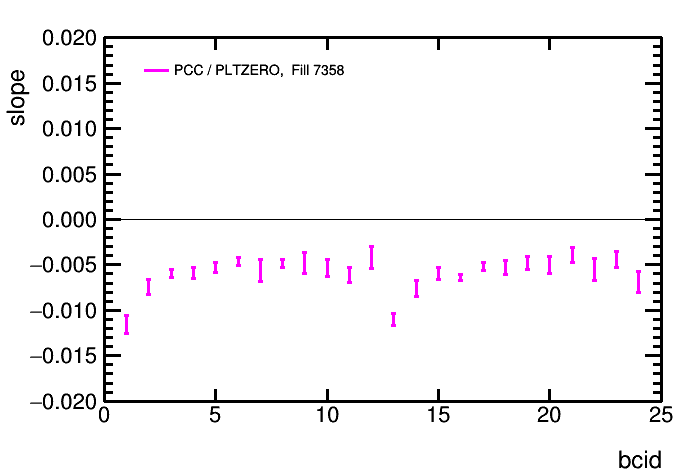
\includegraphics[width=0.47\linewidth]{plots/sbilratios_trains_Fill7358/plot_det_linearity_perbx_slope_7358_plt.png}
    \caption{
      Slope values obtained from the linearity fits for the 24 bunches in the two trains of Fill 7358, in this plot the PCC is compared to the PLTZERO luminometer.
      \label{fig:fill7358trainslope_plt}
    }
  \end{center}
\end{figure}


\clearpage
\begin{figure}[t]
  \begin{center}
    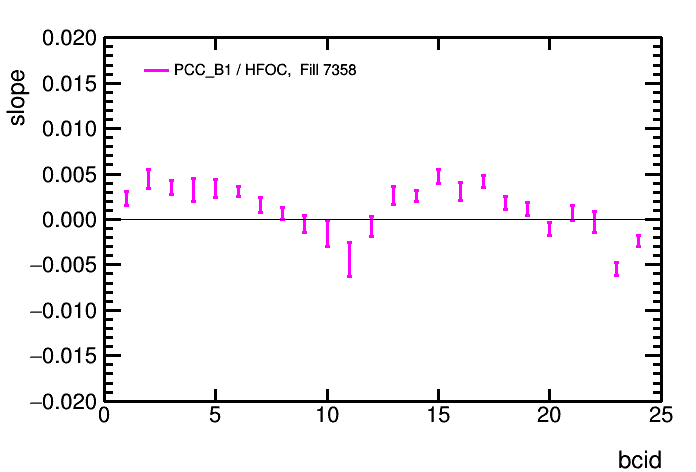
\includegraphics[width=0.32\linewidth]{plots/sbilratios_trains_Fill7358/plot_det_linearity_perbx_slope_7358_B1.png}
    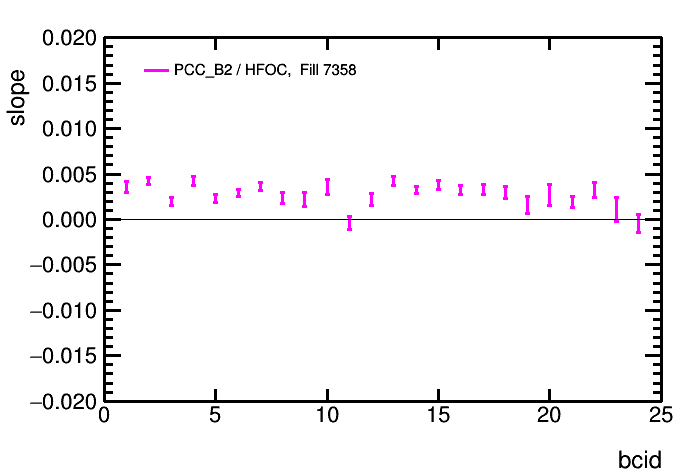
\includegraphics[width=0.32\linewidth]{plots/sbilratios_trains_Fill7358/plot_det_linearity_perbx_slope_7358_B2.png}
    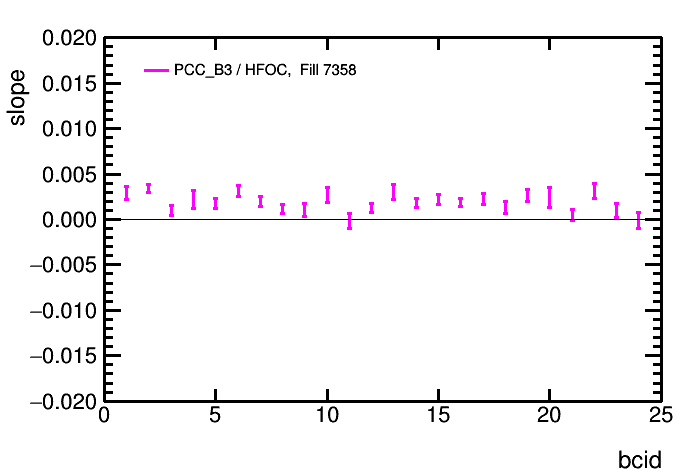
\includegraphics[width=0.32\linewidth]{plots/sbilratios_trains_Fill7358/plot_det_linearity_perbx_slope_7358_B3.png}
    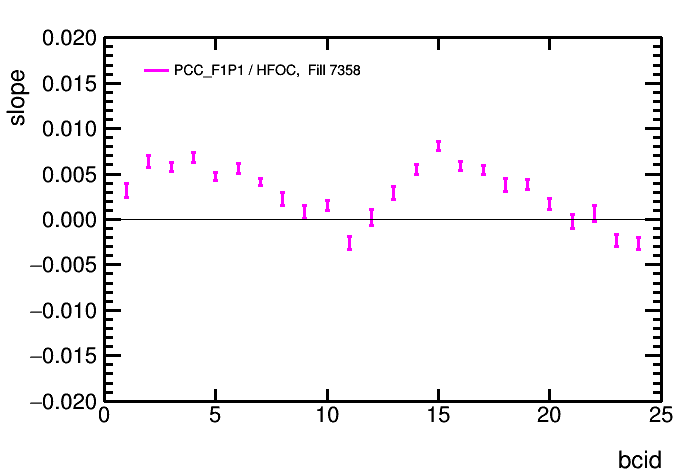
\includegraphics[width=0.32\linewidth]{plots/sbilratios_trains_Fill7358/plot_det_linearity_perbx_slope_7358_F1p1.png}
    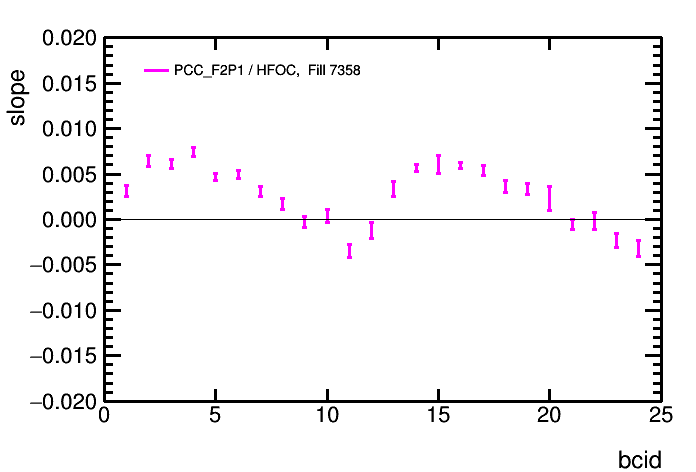
\includegraphics[width=0.32\linewidth]{plots/sbilratios_trains_Fill7358/plot_det_linearity_perbx_slope_7358_F2p1.png}
    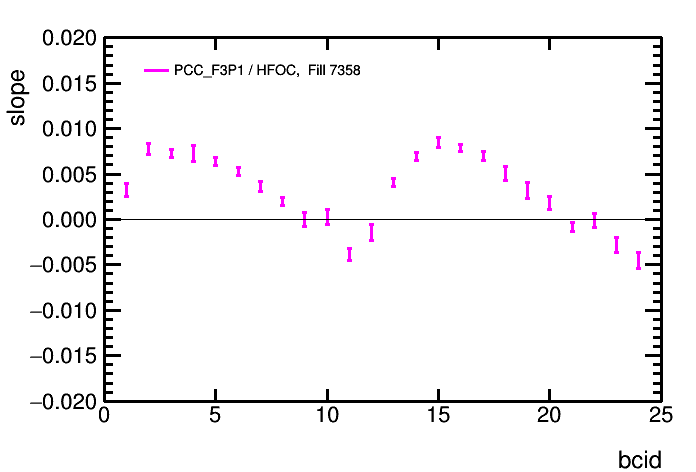
\includegraphics[width=0.32\linewidth]{plots/sbilratios_trains_Fill7358/plot_det_linearity_perbx_slope_7358_F3p1.png}
    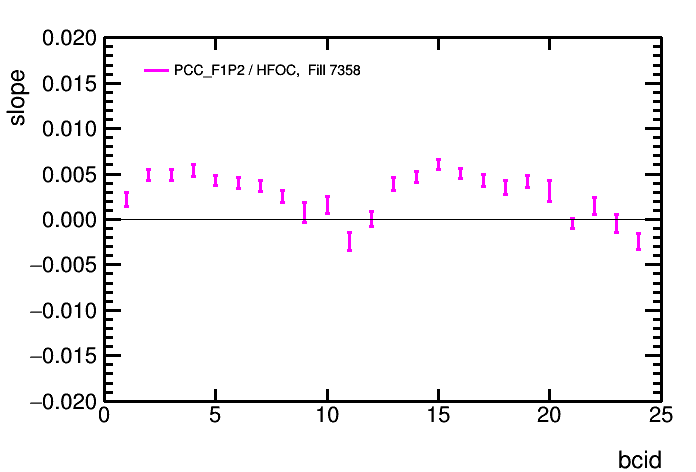
\includegraphics[width=0.32\linewidth]{plots/sbilratios_trains_Fill7358/plot_det_linearity_perbx_slope_7358_F1p2.png}
    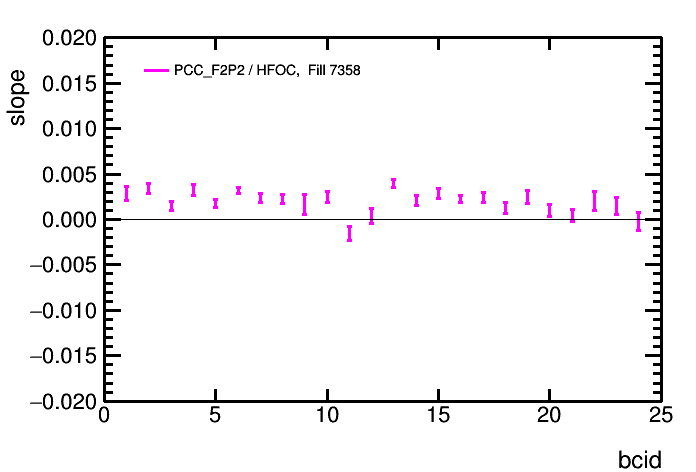
\includegraphics[width=0.32\linewidth]{plots/sbilratios_trains_Fill7358/plot_det_linearity_perbx_slope_7358_F2p2.png}
    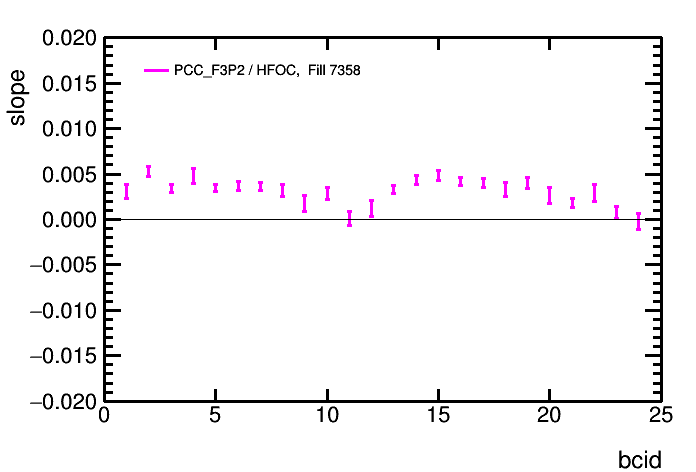
\includegraphics[width=0.32\linewidth]{plots/sbilratios_trains_Fill7358/plot_det_linearity_perbx_slope_7358_F3p2.png}
    \caption{
      Slope values obtained from the linearity fits for the 24 bunches in the two trains of Fill 7358.
      In this plots PCC is shown separately for: \\
      {\bf BPIX} layer 1 (top-left), layer 2 (top-middle), layer 3 (top-right) , \\
      {\bf FPIX Panel 1}:  disk 1 (middle-left), disk 2 (middle-middle), disk 3 (middle-right), and \\
      {\bf FPIX Panel 2}: disk 1 (bottom-left), disk 2 (bottom-middle), disk 3 (bottom-right).
      \label{fig:fill7358trainslope_pccparts}
    }
  \end{center}
\end{figure}
